\section{Memorymanagement}

Es gibt verschiedene Gründe warum nicht immer gleich viel Speicher verwendet wird z.B. da nicht unbegrenzt vorhanden ist.
Speicher wird nur dann verwendet, wenn er wirklich gebraucht wird. 
Das Memorymanagement muss aktiv beachtet werden.
Es wird zwischen automatischen und manuellen Speichermanagement unterschieden. 

\subsection{Automatisch}

Automatisches Speichermanagement wird anhand der Lebenszeit einer Variable festgestellt und während dem Programmieren bereits festgelegt. 
Der Speicher liegt auf dem sogenannten \textbf{Stapel / Stack}.\\
Wird eine Funktion aufgerufen, werden die benötigten Variablen auf dem Stack definiert. 
Ebenso wird eine Returnadresse zur Funktion, die die Funktion aufgerufen hat abgelegt.
Wie die Daten angeordnet werden, ist Architektur-abhängig.
Wird die Funktion wieder verlassen, werden die Variablen vom Stack wieder entfernt und zur aufrufenden Funktion zurückgesprungen.  

\subsection{Manuell/dynamisch}

Man kann auch manuell Speicher anfordern. 
Zum Beispiel, falls zur Compilezeit nicht bekannt ist, wie viel Speicher gebraucht wird.
Dieser Speicher ist auf dem sogenannten \textbf{Haufen / Heap}.\\
Der Heap ist ein Speicherbereich, der vom Betriebssystem bereitgestellt und verwaltet wird.\\
Zur Laufzeit wird Speicher dynamisch angefordert. 
Dieser bleibt so lange belegt bis dieser Manuell wieder freigegeben wird.\\
Es kann aber auch sein, falls der Speicher stark fragmentiert ist, das kein Speicher bereitgestellt werden kann. 
Generell ist bei sehr vollem Speicher das Arbeiten erschwert.

\subsubsection{Memory leaks}

Falls ein Programm unkontrolliert Speicher aufnimmt oder den ihm zur Verfügung gestellte nicht wieder freigibt, spricht man von einem Speicherleck. 
Diese sind zu verhindern da diese zu einer Systemüberlastung und Abstürzen führen.

\example{}
\begin{minipage}{0.5\columnwidth}
  \lstinputlisting[language=C++]{code/04_Memorymanagement/memory_leaks.cpp}
\end{minipage}
\begin{minipage}{0.5\columnwidth}
  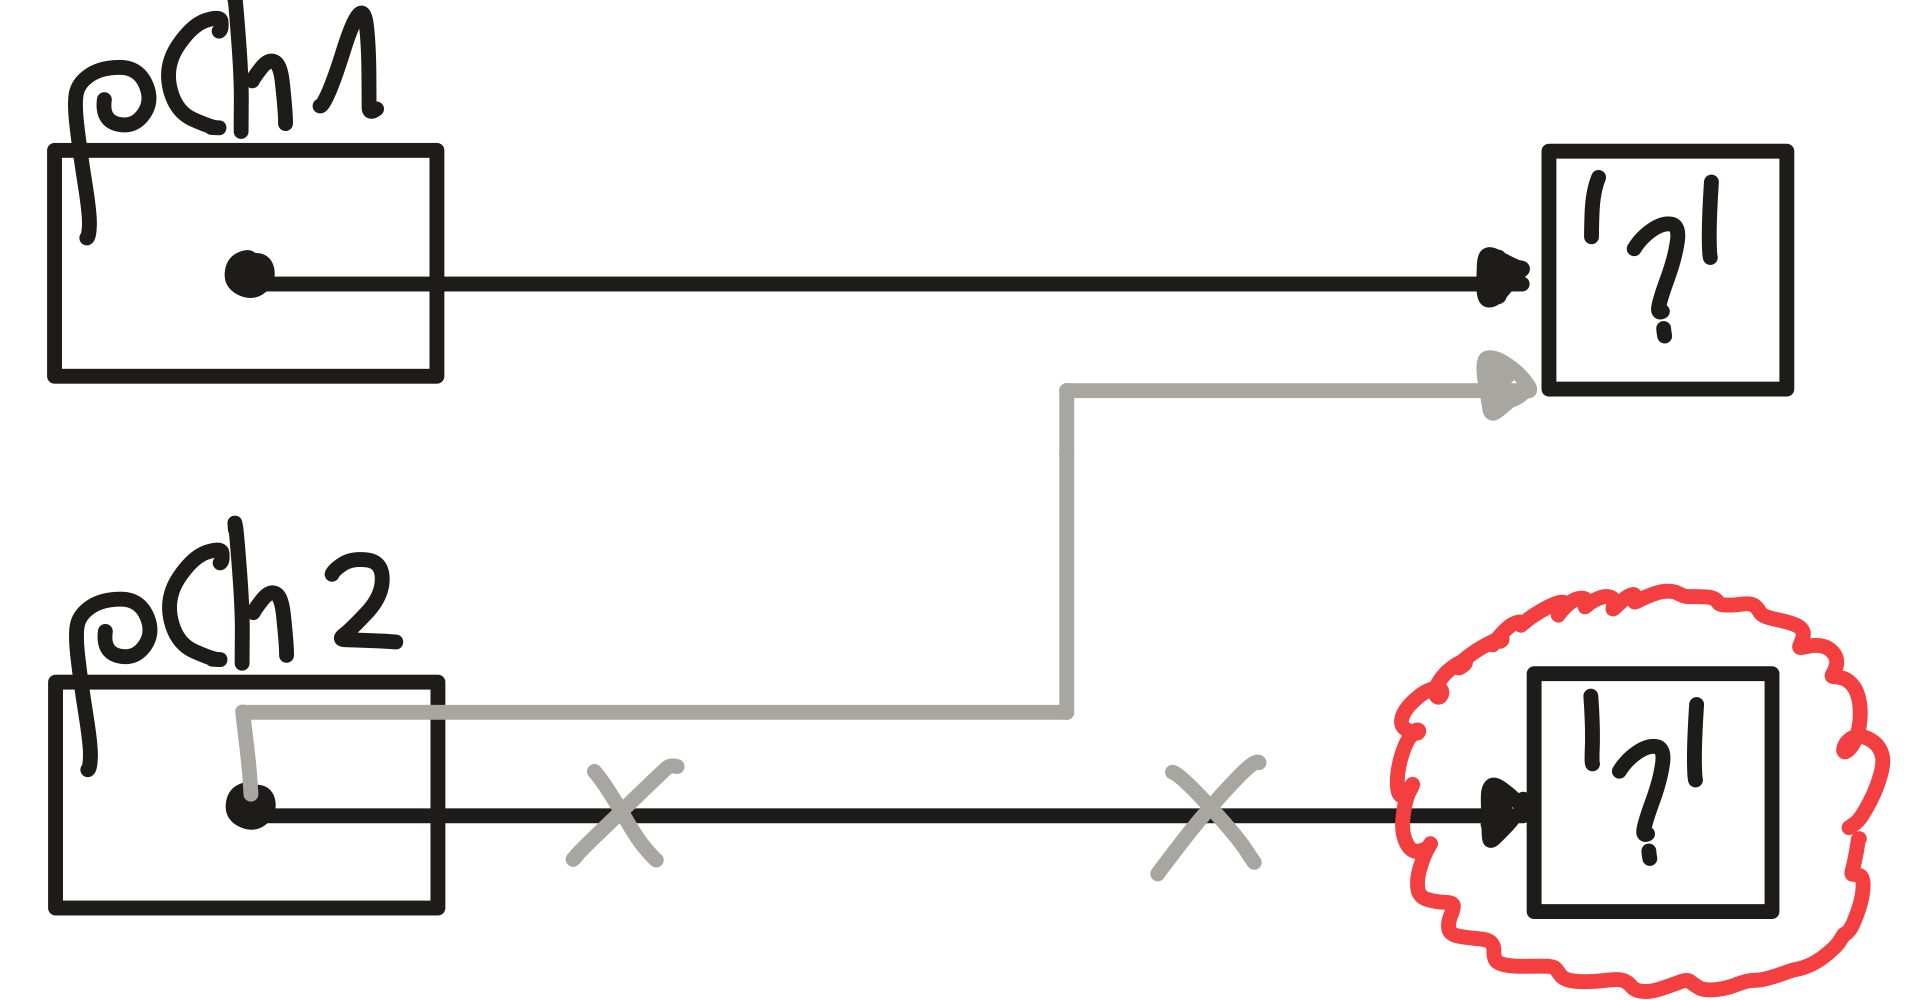
\includegraphics[width=\linewidth]{images/memory_leak.png}
\end{minipage}

\subsection{Speichermanagement funktionen}

Es gibt einige Funktionen für Speichermanagement. In C und C++ sind diese leicht verschieden. 
Generell geben diese einen Pointer zurück, welcher auf freien Speicher zeigt. 
\textbf{Diese müssen immer auf einen Nullpointer geprüft werden, da keine Garantie vorhanden ist, ob überhaupt Speicher vorhanden ist!}
Generell sollte mit solchen Pointer immer misstrauisch gearbeitet werden und nach Abschluss immer wieder freigegeben werden.

\subsubsection{C: \texttt{malloc()},  \texttt{calloc()}, \texttt{free()}}

\textbf{malloc()} gibt einen Voidpointer(pointercasting nicht vergessen) zurück welche auf eine angeforderte Grösse an Bytes Speicher zeigt. 
Der Speicher ist \textbf{nicht} initialisiert
\textbf{calloc()} macht dasselbe, initialisiert aber den Speicher auf 0.\\
\textbf{free()} gibt den Speicherbereich wieder frei.

\lstinputlisting{code/04_Memorymanagement/mem_mngmt_c.c}

Falls kein Speicher allokiert werden kann, wird ein NULL-pointer zurückgegeben.

\subsubsection{C++: \texttt{new}, \texttt{delete}, \texttt{new[]}, \texttt{delete[]} (Operatoren)}

Der \textbf{new}-Operator erstellt ein Pointer welcher auf die mitgegebene Grösse zeigt.

\textbf{new[ ]} macht dasselbe, ausser das dieser ein Array zurückgibt.

\textbf{delete} / \textbf{delete[ ]} gibt den Speicher wieder frei. 
Dieser kann auch auf den Nullpointer ausgeführt werden. 
Dieser ist \texttt{Delete} egal.

\lstinputlisting{code/04_Memorymanagement/mem_mngmt_cpp.cpp}

\subsection{Speicheraufbau}

Der Speicheraufbau bildlich dargestellt sieht ungefähr so aus:

\begin{center}
    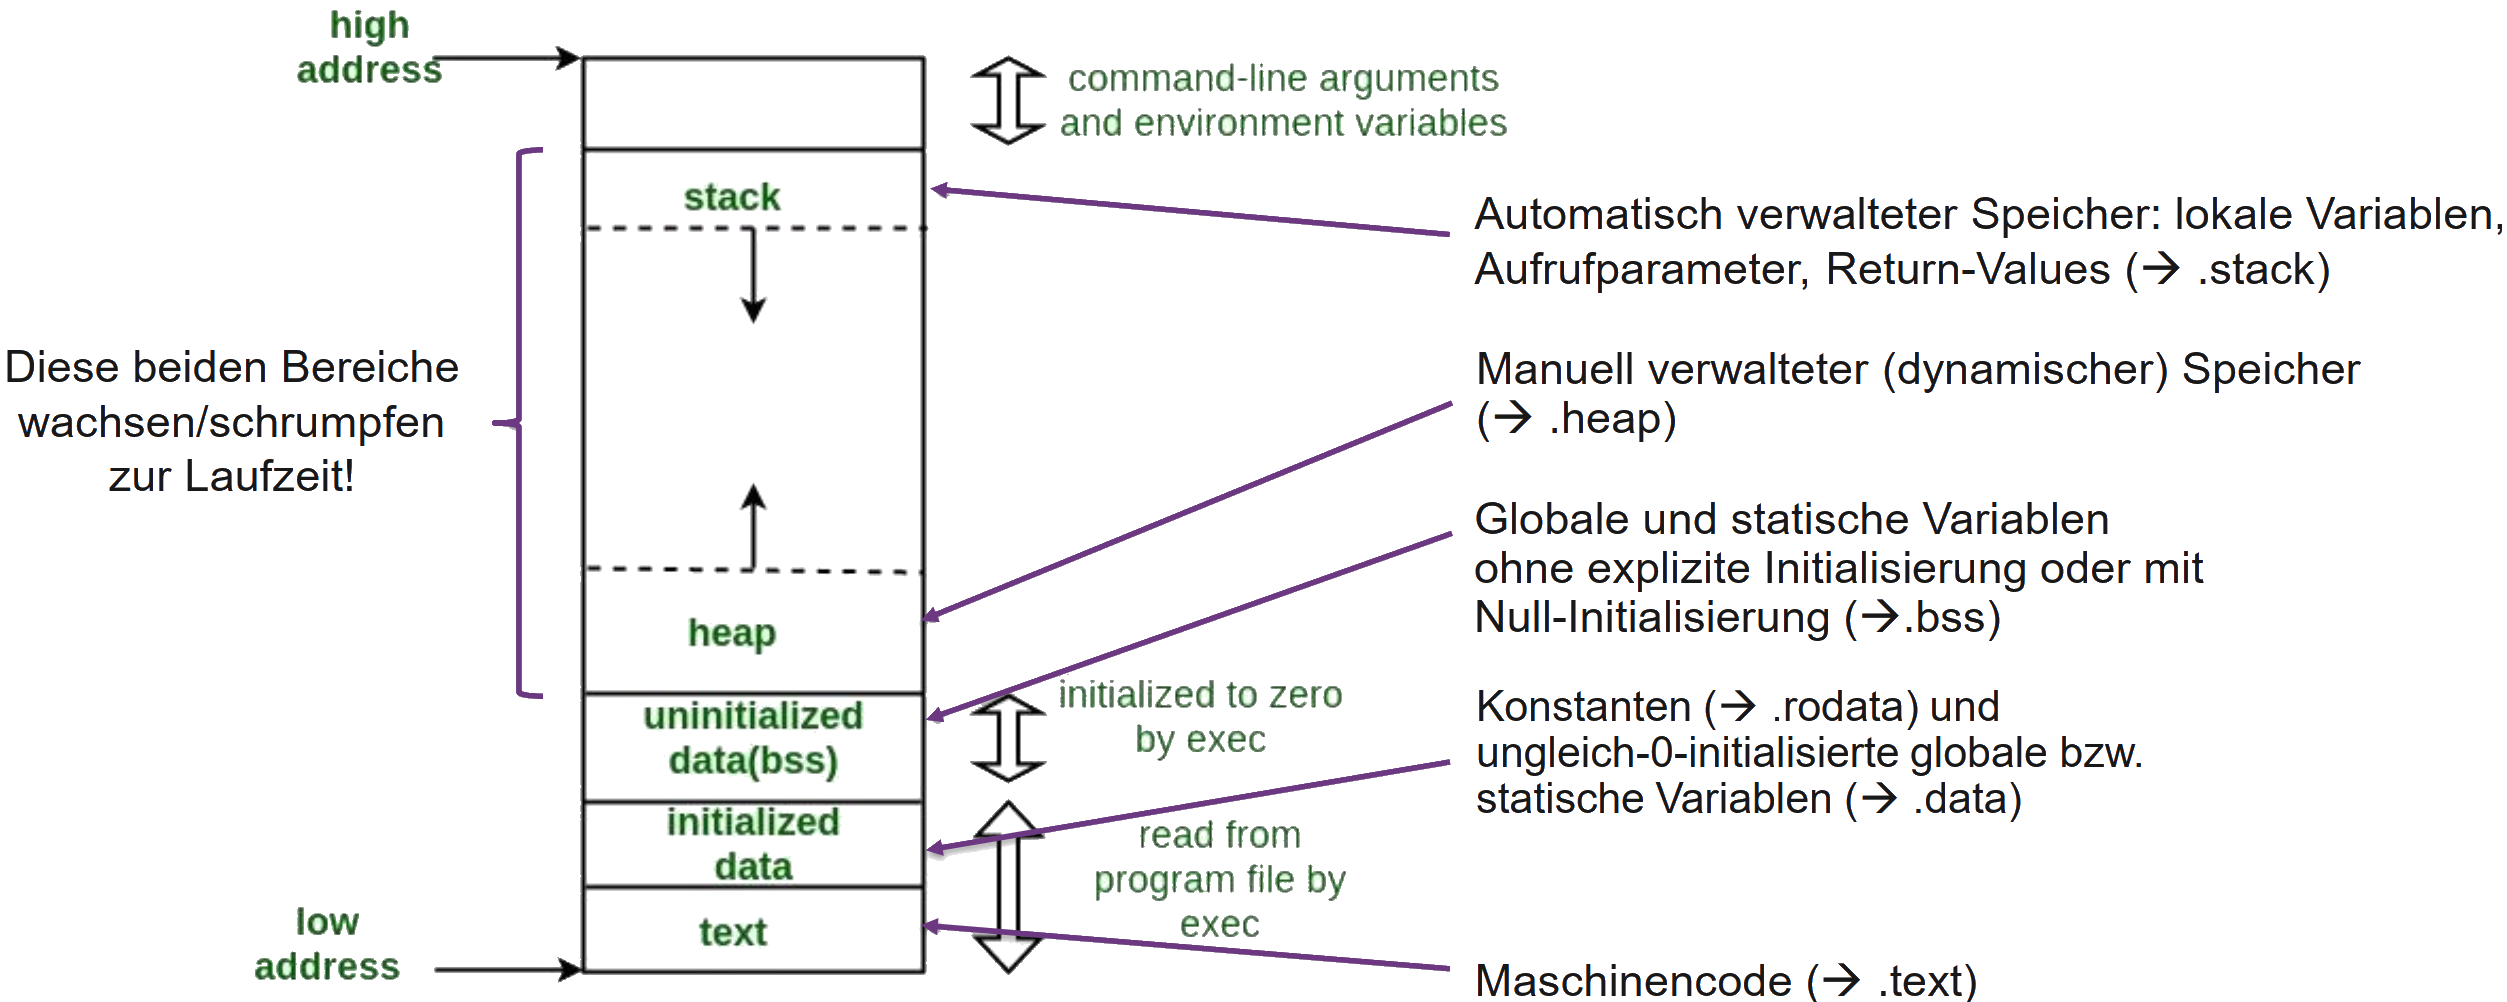
\includegraphics[width=\columnwidth]{images/memorylayout.png}  
\end{center}

Je nach Architektur kann es auch sein, dass die hohen und tiefen Adressen anders herum sind.

\subsection{Referenzen}
Una referenza è un \textbf{alias} (un nome alternativo) per una variabile o una cella di memoria già esistente. Rappresentano una versione più moderna, sicura e ristretta dei puntatori.

\subsubsection{Caratteristiche Principali}
\begin{itemize}
    \item \textbf{Inizializzazione obbligatoria:} Deve essere inizializzata subito: \texttt{int\& r = x;}
    \item \textbf{Immutabilità:} Non può essere modificata per puntare a un altro oggetto dopo la definizione.
    \item \textbf{Sicurezza:} Non possono essere mai non inizializzate e non hanno mai il valore \texttt{nullptr}.
    \item \textbf{Efficienza:} Possono risiedere nei registri della CPU e non occupano sempre memoria fisica. L'operatore \texttt{sizeof()} restituisce la dimensione del tipo a cui la referenza punta.
    \item \textbf{Sintassi:} Vengono utilizzate come variabili normali, senza necessità di dereferenziazione.
    \item \textbf{Limitazione con gli Array:} Le referenze non possono essere usate per scorrere gli array tramite aritmetica (incremento/decremento). Per questo scopo, i \textbf{puntatori} rimangono indispensabili.
\end{itemize}

\subsubsection{Confronto: Value vs Reference}
\begin{center}
\begin{tabular}{@{}lll@{}}
\toprule
\textbf{Caratteristica} & \textbf{Call by Value} & \textbf{Call by Reference} \\ \midrule
Copia dei dati          & Sì (costoso per oggetti grandi) & No (passa l'alias) \\
Modifica originale      & No                             & Sì \\
Sintassi                & \texttt{void f(int a)}         & \texttt{void f(int\& a)} \\ \bottomrule
\end{tabular}
\end{center}

\subsubsection{Best Practices}
L'utilizzo delle referenze riduce drasticamente i rischi di errori rispetto ai puntatori. Tuttavia, i puntatori rimangono necessari in casi specifici:
\begin{itemize}
    \item \textbf{Gestione degli Array:} Un array "decade" naturalmente in un puntatore al suo primo elemento (\textit{pointer decay}), rendendo i puntatori lo strumento standard per iterare o manipolare blocchi di memoria contigui.
    \item \textbf{Programmazione Low-level:} Necessaria per l'interazione diretta con l'hardware o allocazione dinamica manuale (\texttt{new}/\texttt{delete}).
\end{itemize}

\lstinputlisting{code/04_Memorymanagement/referenz.cpp}

\subsection{Speicherplatzbedarf von Objekten}

Eine Unterklasse braucht immer mindestens so viel speicher wie eine Oberklasse.

\subsubsection{Zuweisungen}

Zuweisungen von Oberklasse zu Unterklasse sind in der regel möglich da alle geerbten Attribute ja vorhanden sind. 
Umgekehrt geht das allerdings nicht, da der Speicher dafür nicht initialisiert ist.

\subsubsection{Slicing Problem}

\begin{itemize}
    \item \textbf{Definizione:} Si verifica quando un oggetto di una sottoclasse viene passato \textbf{per valore} a una funzione che si aspetta la superclasse.
    \begin{itemize}
        \item Viene invocato il \textit{Copy-Constructor} della superclasse.
        \item Solo la parte "base" dell'oggetto viene copiata; le estensioni della sottoclasse vengono perse (slicing).
    \end{itemize}
    \item \textbf{Conseguenza:} All'interno della funzione, l'oggetto si comporta esclusivamente come un'istanza della classe base, perdendo ogni comportamento polimorfico.
    \item \textbf{Soluzione:} Utilizzare sempre il passaggio \textbf{per referenza} (\texttt{const T\&}) o tramite puntatori. Questo preserva l'integrità dell'oggetto originale e permette il corretto funzionamento dei metodi \texttt{virtual}.
\end{itemize}

\subsection{Type Casting}\vspace{-1em}

\begin{center}
    \rotatebox{90}{%            
    \resizebox{1.5 \columnwidth}{!}{%
    \begin{tabular}{|c|l|l|l|}
        \hline
        {\color{blue} Cast:} &
          \multicolumn{1}{c|}{{\color{blue} Anwendungsbereiche}} &
          \multicolumn{1}{c|}{{\color{blue} Wissenswertes}} &
          \multicolumn{1}{c|}{{\color{blue} Beispiele}} \\ \hline
        {\color{blue} \begin{tabular}[c]{@{}c@{}}implizit: \\ kein Cast\end{tabular}} &
          \begin{tabular}[c]{@{}l@{}}• Numerische Typen u. bool\\ (ggf. mit Warnung, falls Wertebereich\\ möglicherweise nicht ausreicht)\\ • Objektinstanzen einer Unterklasse in\\ einer Variablen vom Typ der\\ Oberklasse speichern (Upcast).\\ • Pointertypen, deren Umkonvertierung\\ «ungefährlich» ist – die genauen\\ Regeln sind ziemlich kompliziert.\end{tabular} &
           &
          \begin{tabular}[c]{@{}l@{}}1. {\color{codeGreen}signed char} a = 1;\\ {\color{codeGreen}int} b = a;\\ \\ 2. {\color{codeGreen}int} a = 1;\\ {\color{codeGreen}char} b = a; {\color{blue}// ggf. mit Warnung}\\ \\ 3. Bird b;\\ Animal a = b; {\color{blue}// Upcast: a ist ein Animal}\end{tabular} \\ \hline
        {\color{blue} static} &
          \begin{tabular}[c]{@{}l@{}}• Alles, was implizit möglich ist,\\ unterdrückt dabei etwaige Warnungen.\\ • Pointer- und Referenz-Typen auf\\ Instanzen von Ober- und\\ Unterklassen in beide Richtungen\\ umwandeln: Upcast und\\ Downcast (\textbf{ohne Typprüfung} zur\\ Laufzeit, Auswertung\\ ausschliesslich zur \textbf{Compilezeit})\end{tabular} &
          \begin{tabular}[c]{@{}l@{}}Per convertire un tipo intero più \\ grande in uno più piccolo, il \\ compilatore semplicemente "taglia" \\ i bit in eccesso, mantenendo solo \\ quelli meno significativi (LSB).\end{tabular} &
          \begin{tabular}[c]{@{}l@{}}1. {\color{codeGreen}int} a = 1;\\ {\color{codeGreen}char} b = {\color{codeGreen}static\_cast}\textless{}{\color{codeGreen}char}\textgreater{}(a);\\ 2. Bird* b = {\color{codeGreen}new} Bird;\\ Animal* a = b; {\color{blue}// geht implizit!}\\ Bird* c = {\color{codeGreen}static\_cast}\textless{}Bird*\textgreater{}(a);\\ {\color{blue}/* Braucht einen down-Cast} , \\ {\color{codeGreen}weil nicht jedes Animal ein Bird ist!*/}\end{tabular} \\ \hline
        {\color{blue} dynamic} &
          \begin{tabular}[c]{@{}l@{}}• Pointer- und ReferenzTypen auf \\ Instanzen von\\ \textbf{polymorphen} Ober- und\\ Unterklassen in beide\\ Richtungen umwandeln:\\ Upcast und Downcast (\textbf{mit}\\ Typprüfung per RTTI zur\\ Laufzeit)\end{tabular} &
          \begin{tabular}[c]{@{}l@{}}Unterstützt ausserdem einen\\ Upcast für Pointer- und\\ Referenztypen auf nichtpolymorphe Klassen\\ (normalerweise machen wir dies aber \\ implizit oder verwenden einen static\_cast!)\\ Falls der dynamic\_cast \textbf{fehlschlägt}, liefert \\ er bei Pointer-Typen den Wert\\ \textbf{nullptr}, bei Referenzen wird\\ eine \textbf{std::bad\_cast-Exception} geworfen\end{tabular} &
          \begin{tabular}[c]{@{}l@{}}Animal* a = {\color{codeGreen}new} Ant;\\ Bird* b = {\color{codeGreen}dynamic\_cast}\textless{}Bird*\textgreater{}(a);\\ {\color{blue}/* Der Dynamic Cast wird}\\ {\color{blue}immer zur Laufzeit ausgewertet.  dh:}\\ {\color{blue}b ==nullptr */}\end{tabular} \\ \hline
        {\color{blue} const} &
          \begin{tabular}[c]{@{}l@{}}verändert die \texttt{constness} und/oder\\ \texttt{volatile-ness} des\\ Ziels eines Pointer oder Referenz Typs.\end{tabular} &
           &
          \begin{tabular}[c]{@{}l@{}}{\color{codeGreen}const int} val = 10; \\ {\color{codeGreen}const int} *ptr = \&val; \\ {\color{codeGreen}int} *ptr1 = {\color{codeGreen}const\_cast} \textless{}{\color{codeGreen}int} *\textgreater{}(ptr);\end{tabular} \\ \hline
        {\color{blue} reinterpret} &
          \begin{tabular}[c]{@{}l@{}}• Konvertiert zwischen beliebigen Pointer-Typen \\ sowie zwischen beliebigen Pointer und int-Typen \\\textbf{ohne Typprüfung}.\\ • Kann auch mit Referenz-Typen\\ umgehen.\end{tabular} &
          \begin{tabular}[c]{@{}l@{}}Achtung: erzeugt\\ plattformspezifisches Verhalten\end{tabular} &
          \begin{tabular}[c]{@{}l@{}}Animal* a = {\color{codeGreen}new} Ant;\\ \\ {\color{codeGreen}uint8\_t}* b =\\ {\color{codeGreen}reinterpret\_cast}\textless{}{\color{codeGreen}uint8\_t}*\textgreater{}(a);\end{tabular} \\ \hline
        \end{tabular}%
    }
    }          
\end{center}

Die C Syntax für Casting sollte nicht mehr verwendet werden da meistens nicht optimales verhalten. 

\subsection{Templates}

\begin{itemize}
\item \textbf{Indipendenza dal tipo:} Consentono di scrivere codice generico utilizzando dei \textbf{placeholder} (segnaposti) al posto di tipi specifici.
\item \textbf{Sicurezza dei tipi (Type Safety):} A differenza del C 
(\lstinline|void*|), i template garantiscono un controllo dei tipi tramite \textit{early binding} in fase di compilazione.
\item \textbf{Parametri di istanziazione:} Oltre ai tipi, è possibile 
passare anche delle \textbf{costanti} come parametri del template 
\item \textbf{Versatilità:} Possono essere applicati sia a \textbf{classi} che a 
\textbf{funzioni}.
\item \textbf{Valutazione a tempo di compilazione:} Il compilatore genera il codice 
effettivo durante la fase di \textbf{compile-time}.
\item \textbf{Struttura e File:} Richiedono dichiarazione, definizione e parametri; 
solitamente vengono \crd{definiti interamente negli \textbf{header file} (.h / .hpp).}
\item \textbf{Generazione del codice:} Il compilatore crea una copia separata della 
funzione o classe per ogni \textbf{diverso tipo} utilizzato.
\item \textbf{Zero Dead Code:} Se un template non viene mai utilizzato nel codice, 
non viene generata alcuna istruzione nel binario finale
\item \textbf{Footprint di memoria e Code Bloat:} L'istanziazione per molteplici tipi, 
oppure l'uso eccessivo della keyword \lstinline|inline| per definizioni lunghe, 
può causare \textit{code bloat}.
\end{itemize}

\subsubsection{Implementation}

Die Typendefinitionen sind dann durch das T zu ersetzen. 

\lstinputlisting{code/04_Memorymanagement/templatesswap.cpp}\vspace{-1.5em}

\begin{center}
  \cor{As the dimension of the paramters is unknow ALWAYS use references}
\end{center}

\subsubsection{Syntax}

\lstinputlisting{code/04_Memorymanagement/templatesyntax.cpp}\vspace{-0.5em}

\subsubsection{Instanziierung}

L'istanziazione è il processo con cui il compilatore genera codice macchina concreto\smallbreak

\begin{itemize}
    \item \textbf{Implicita:} compilatore deduce il tipo dai parametri passati 
    \textbf{Nota bene:} il tipo di ritorno non viene mai considerato per la deduzione
    \item \textbf{Esplicita:} Il tipo viene specificato manualmente tra parentesi angolari 
\end{itemize}\smallbreak

\textbf{Klassentemplates} (\verb|<>| obbligatori):\\
tipo sempre specificato per permettere al compilatore di determinare l'ingombro in memoria.\\
\lstinline[language=C++]|Stack<int, 10> s1; // Istanzia uno Stack di 10 interi|

\textbf{Funktionstemplates} (\verb|<>| opzionali se deducibili):\\
Se il tipo è chiaro dai parametri, le parentesi angolari possono essere omesse.\\
\lstinline[language=C++]|int i = minimum(iF, size); // Deduzione implicita del tipo int|
\lstinline[language=C++]|int i = minimum<int>(iF, size); // Qualificazione esplicita|

\subsubsection{Overloading}

I template di funzione possono essere sovraccaricati (overloaded) con altri template o con funzioni "normali". In caso di chiamate omonime, il compilatore valuta le funzioni compatibili, istanzia quelle dei template, le aggiunge alle funzioni normali disponibili e infine seleziona la variante che offre il \textit{match} migliore con i tipi dei parametri passati.

\subsubsection{Kompilierung und Code-Organisation}
\begin{itemize}
    \item \textbf{Header-Only:}  il compilatore deve 'vedere' la definizione per ogni 
    traduzione. Lo svantaggio principale è l'\textbf{aumento dei tempi di compilazione} 
    \item \textbf{Explicit Instantiation (.cpp):} Per ridurre i tempi di compilazione, 
    è possibile spostare la definizione in un file \verb|.cpp| e forzare l'istanziazione 
    per tipi specifici (es. \lstinline|template class Stack<int>;|). 
\end{itemize}

\section{Exceptions (Ausnahmen)}
\begin{itemize}
    \item \textbf{Error (Fehler):} Errore di implementazione. Dovrebbe essere rimosso durante il testing/verifica.
    \item \textbf{Exception (Ausnahme):} Condizione anormale che può verificarsi a runtime (es. file non trovato, timeout di rete).
\end{itemize}


\subsection{Meccanismo: Throw e Catch}
Un'eccezione è un oggetto lanciato con la keyword \texttt{throw} e intercettato da un blocco \texttt{catch}.

\begin{itemize}
    \item \textbf{Throw by value:} Le eccezioni dovrebbero sempre essere lanciate per valore.
    \item \textbf{Catch by const reference:} Per evitare copie inutili e il problema dello \textit{slicing} degli oggetti, intercettare sempre per riferimento costante.
    \item \textbf{Stack Unwinding:} lanciata un'eccezione, il programma distrugge 
    automaticamente tutti gli oggetti (chiama i distruttori) e salta 
    \textbf{al primo handler compatibile}.
\end{itemize}

\lstinputlisting[language=C++]{code/04_Memorymanagement/exceptionGenerellSyntax.cpp}\vspace{-1em}

\subsection{Propagazione (Exception Propagation)}
Se un'eccezione non viene gestita localmente, può essere passata "verso l'alto" (es. fino al livello applicativo) dove può essere presa una decisione sensata (Grundsatz: gestire solo ciò che si può decidere).
\begin{itemize}
    \item All'interno di un blocco \texttt{catch}, l'istruzione \texttt{throw;} (senza argomenti) ri-lancia l'eccezione corrente alla funzione chiamante.
\end{itemize}

\subsection{Gerarchia e Ordine dei Catch}
In C++, le eccezioni sono organizzate gerarchicamente sotto la classe base \texttt{std::exception} (definita in \texttt{<exception>}).

\begin{itemize}
    \item \textbf{logic\_error: \crd{DA NON USARE}} Errori prevenibili in fase di sviluppo
    \item \textbf{runtime\_error:} Errori non prevedibili dovuti a eventi esterni\\
    (es. \texttt{overflow\_error}, \texttt{system\_error}, \crd{includere \texttt{stdexcept}}).
\end{itemize}

\medbreak

\textbf{\color{orange}Regola cruciale:} Gli handler devono essere ordinati dal più specifico al più 
generico nel codice. \texttt{std::exception} o il catch-all \texttt{...} deve essere l'ultimo.

\begin{lstlisting}{language=C++}
catch(...) {
  // Catch everything
}
\end{lstlisting}

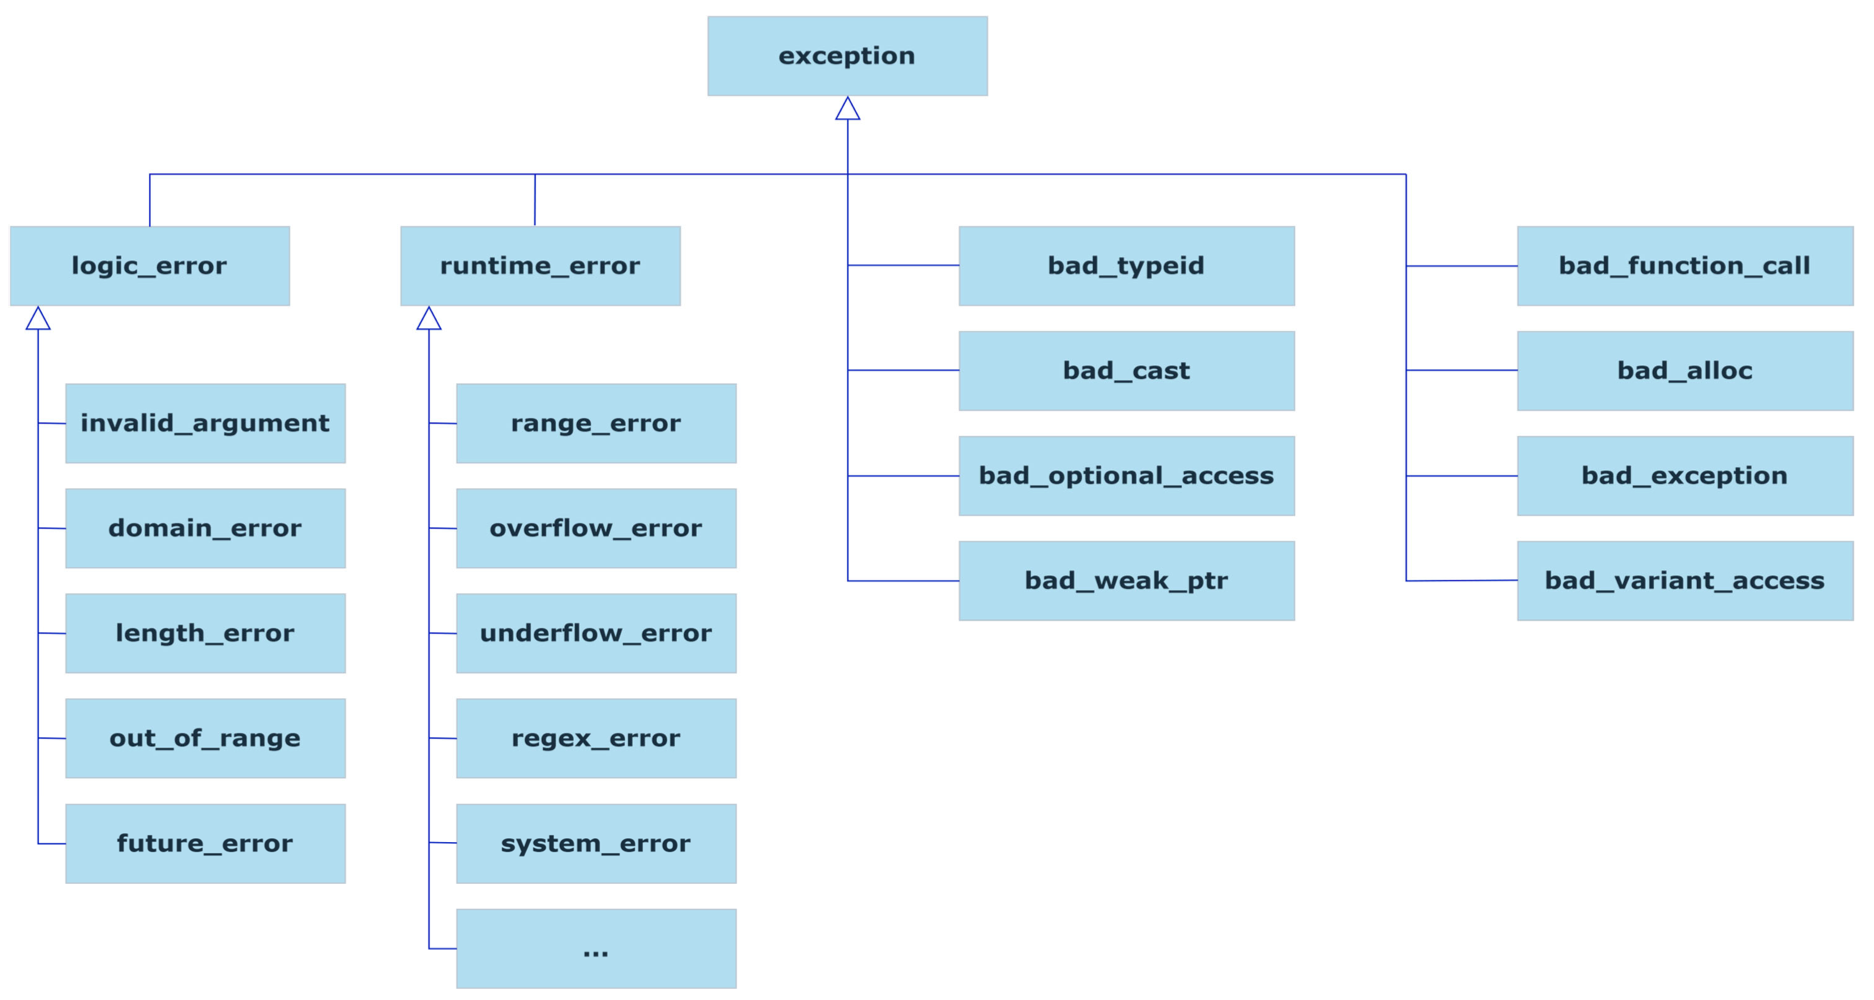
\includegraphics[width=\linewidth]{images/exception_hierarchie.png}

\example{}
\lstinputlisting[language=C++]{code/04_Memorymanagement/catchcatcher.cpp}\vspace{-1em}

\subsection{Eccezioni non gestite}
Se non viene trovato alcun handler nel \textit{Call Stack}:


\begin{enumerate}
    \item Viene chiamata la funzione \texttt{std::terminate}.
    \item \texttt{std::terminate} richiama un \texttt{terminate\_ handler} (di default \texttt{std::abort}).
    \item Il programma termina bruscamente (no esecuzione dei distruttori)
\end{enumerate}\smallbreak

È possibile personalizzare questo comportamento tramite \texttt{std::set\_terminate()}.

\subsection{noexcept}
\begin{itemize}
    \item \textbf{noexcept:} Introdotto con C++11, indica che una funzione garantisce di non lanciare eccezioni. È utile per l'ottimizzazione del compilatore.
    \item \textbf{Operatore noexcept(expr):} Restituisce \texttt{true} se l'espressione è specificata come \texttt{noexcept}.
\end{itemize}

\lstinputlisting[language=C++]{code/04_Memorymanagement/noexcept.cpp}\vspace{-1em}

\subsection{C++ e Low-Level Exceptions}
A differenza di Java o C\#, il linguaggio C++ \textbf{non} effettua il \textit{mapping}
automatico delle eccezioni di basso livello (come la divisione per zero) in eccezioni 
del linguaggio.
\smallskip

Handling con \texttt{catch(...) \{ \}} 

\section{STD Library}
\subsection{array}
\begin{itemize}
\item \textbf{Definizione:} \texttt{std::array<T, size>} è un contenitore a dimensione fissa implementato come classe template.
\item \textbf{Dimensione:} A differenza dei classici array in stile C, \texttt{std::array} conosce la propria dimensione tramite la funzione membro \texttt{.size()}.
\item \textbf{Accesso ai dati:} È possibile accedere agli elementi utilizzando la classica notazione a parentesi quadre \texttt{[]}.
\item \textbf{Sicurezza:} Il metodo \texttt{.at()} fornisce un accesso sicuro con controllo dei limiti, lanciando un'eccezione \lstinline|std::out_of_range| in caso di accesso non valido.
\item \textbf{Integrazione:} Funziona in modo ottimale con le moderne funzionalità del C++, inclusi i cicli \textit{range-based for}.
\end{itemize}

\subsection{vector}
std:vector ist ein Klassentemplate welches die Kapazität selbständig bei Bedarf erweitert.
\lstinputlisting{code/04_Memorymanagement/vector.cpp}